\documentclass[letterpaper, 11pt]{article}
\usepackage[utf8]{inputenc}
\usepackage{mathptmx}
\usepackage{natbib}
\usepackage[top=1in, bottom=1.25in, left=1.25in, right=1.25in]{geometry}
\usepackage{enumitem}
\usepackage[usenames,dvipsnames]{xcolor}
\usepackage{hyperref}
\hypersetup{colorlinks=true,allcolors=MidnightBlue}
\usepackage{titlesec}
\usepackage{graphicx}
\usepackage{wrapfig}
\usepackage{enumitem}
\usepackage{array}
\usepackage{booktabs}
\usepackage{float} 

%%%%%%%%%%%%%%%
%% FEEL FREE TO ADD MORE PACKAGES %%% 
%%%%%%
%%% LaTeX 
%% https://www.overleaf.com/learn/latex/Learn_LaTeX_in_30_minutes
%% https://www.overleaf.com/learn/latex/Positioning_images_and_tables 

%%% TODO: change TOPIC to your title
\title{Literature Review: How Question-Answering Models Handle Unanswerable Queries}
%%% TODO: change YOURNAME and yournetid to your name and NetId
\author{Samuel Schreiber,\\ srs17@illinois.edu}

\begin{document}

\maketitle

\begin{abstract}
This review covers four papers that discuss how question-answering models are trained and evaluated on unanswerable questions. It seeks to define what an unanswerable question is, how models can handle them without hallucination,
and how performance can be evaluated. It covers specific types of unanswerable questions, including those with `questionable assumptions' in an open-domain setting, plausible unanswerable questions in a closed-domain setting
where the question cannot be answered based on some provided context, and adversarial attacks where the question is deliberately crafted to trick the model into providing a bogus answer.
Finally, it examines information-seeking questions where the answer could be found across many contexts, and the subtasks of paragraph retrieval and answerability detection. 
\end{abstract}

\section{Introduction}
\label{sec:introduction}

Question-Answering models have made significant progress in recent years, with models like GPT-3 and BERT achieving human-level performance on many question-answering tasks. Performance for these models is often evaluated over good-faith, well-formulated questions with answers that are present either in an \textbf{open or closed domain setting}  (see \ref{sec:open-vs-closed-domain-question-answering}). In some cases, such as in a closed-domain setting where users ask questions based on specific contexts (such as an article), 
models that appear to perform well may simply be matching questions to the \textbf{context span} (or snippet) that is most related to the question. For example, if the context is \textit{`... The age of the Earth is 4.543 billion years old. ...'}, to answer the question of \textit{`How old is the Earth?'}, the model may simply match the question to the context span \textit{`Earth is 4.543 billion years old'}.
In such case, there is no reason to believe the model has any true natural language understanding of the question; it could simply be pattern-matching based on some similarity metric. Moreover, the context span may simply refer to the entities or concepts in the question without providing any meaningful answer. For this reason, it is important to reassess how models are trained and evaluated so that they can handle unanswerable questions, provide more meaningful answers beyond matching the question to a context span, and provide more reasonable performance metrics
more reflective of the model's performance in the real world. But what is an unanswerable question, and how can models learn to detect them to provide a reasonable response rather than hallucinating (or making up some spurious) answers? Finally, how can we evaluate the performance of models on such questions?
These are the questions we seek to clarify in this review.

\section{Know what you don't know: Unanswerable questions}
\label{sec:know-what-you-dont-know} 

% why the paper was chosen
% 4 pts It was very clear for each of the papers that were discussed in depth why it was included and what the reader should care about them.
\subsection{Motivation}
This paper \citep{knowwhatyoudont} was selected because it points out a common flaw in evaluating question-answering models and that many models only perform well because the question-answering datasets only contain answerable questions or easily identifiable unanswerable questions,
resulting in a biased view of the models' performance. It raises awareness about the need to think critically about how models are evaluated and how biases that may be imposed on the test dataset may affect the models' performance.
This paper is relevant to our overarching question because it identifies a new type of unanswerable question, and offers a new dataset to train and evaluate models on unanswerable questions to avoid hallucinating an answer.

% background
% 4 pts The paper provided enough technical background to help the reader understand the papers that are discussed.
\subsection{Background Knowledge}
\subsubsection{SQuAD 1.1 Dataset}
\label{sec:squad-1.1}

This paper discusses \textbf{SQuAD} (Stanford Question-Answering Dataset), a commonly used dataset used to train and evaluate question-answering models.
It consists of many question-answer pairs, where the model is provided a context with a set of questions and is expected to provide the respective answers.
The models' answers are compared to the ground truth answers provided in the dataset to determine if the answer was relevant or not (see the section~\ref{sec:f1-score} for more information about model evaluation). 
It is vital to note that the dataset only contains answerable questions.
\\

% sub subsection
\noindent
Here is an example of a question from the SQuAD dataset:
\begin{quotation}
    \noindent
    \textbf{Context:}
    The Normans were originally Viking raiders from Scandinavia who settled in the region of France known as Normandy. They became known for their military prowess and eventually played a significant role in the history of England, particularly after their victory in the Battle of Hastings in 1066.
    \\
    \\
    \textbf{Question 1:} Where did the Normans settle in France?
    \\
    Answer: Normandy
    \\
    \\
    \textbf{Question 2:} When was the Battle of Hastings?
    \\
    \textbf{Answer:} 1066
\end{quotation}


\noindent Notice the context provides a set of facts, and all the question's answers can be found in the context in contrast to section~\ref{subsec:question-answering-with-questionable-assumptions} where specific context is not provided.
Humans may manually determine if the answer a model generates was correct based on the context, or determine if the question was correctly labeled as unanswerable.


\subsubsection{F1 Score}
\label{sec:f1-score}
A common way to evaluate the performance of a question-answering model is to calculate the \textbf{F1 score} which is a harmonic mean of the \textbf{precision and recall} of the models' answers.
In this case, the precision is the percentage of tokens (often words or sub-words) in the models' answer that are also in the ground truth answer, and the recall is the percentage of tokens in the ground truth answer that are also in the models' answer.
Moreover, precision tells us how much of the generated answer is correct, and recall tells us about the coverage of the generated answer.

\subsubsection{Development, Test, and Training Sets}
\label{sec:development-test-training-sets}
The SQuAD dataset is split into three sets: \textbf{the training set, the development set, and the test set}. The training set is used to train the model, the development is used during training to tune the model's hyperparameters and check the model's performance during training, and the test set is used to evaluate the model's performance after the model's training has finished.
It is essential that the final model not be trained on the development or test sets to avoid invalid performance evaluation.
% subsection overview of paper
% 12 pts The author made an attempt to describe the papers in their own words, and the description was very clear. The reader can follow completely, and is getting all the important details.
\subsection{Overview}
The paper discusses how the SQuAD 1.1 dataset only contains answerable questions and models that perform well may not have any true understanding of the question.
Models that perform well may simply match a question to the span of the context that is most related to the question rather than understanding the question and providing a meaningful answer.
To address this shortcoming, the authors propose \textbf{SQuAD 2.0}, which augments the original dataset with over 50,000 unanswerable questions.
The authors show that state-of-the-art question-answering models in 2018, at the time of the paper's publication, achieve an F1 score of 66.3\% on SQuAD 2.0, compared to 85.8\% on SQuAD 1.1, highlighting the models' struggle with unanswerable questions.
Furthermore, the performance of state-of-the-art models on SQuAD 1.1 is 5.4 points worse than humans, while the performance on SQuAD 2.0 is 23.2 points worse than humans, further demonstrating the models' shortcoming's in handling unanswerable questions.


\subsubsection{Data Collection}
The authors collected unanswerable questions by asking crowd workers to write unanswerable questions for selected SQuAD 1.1 contexts. They were instructed
to pose five questions per context that referenced entities or concepts that were present but not directly answerable by the context. The questions must have also been plausibly answerable by a human. There were some filters
in place to remove questions from humans who did not produce quality questions. These questions were then added to the SQuAD 1.1 dataset to create SQuAD 2.0.
\\
The authors used crows workers to have humans answer questions from SQuAD 2.0 development and test sets to confirm that the dataset was clean. They were exposed to mixed sets of unanswerable and answerable questions and were asked to either 
underline the answer in the context or mark it as unanswerable. If more than half of workers marked a question as unanswerable, it was labelled as unanswerable. 93\% of the questions
that were marked as unanswerable were truly unanswerable. 

% interpretation
% 4 pts The author attempted to provide a sufficient amount of further interpretation, analysis or discussion of the papers.
\subsection{Contribution, Critique and Analysis}
The curation of the SQuAD 2.0 dataset is a significant contribution to question-answering research. It highlights a bias in the original SQuAD 1.1 dataset that results in less meaningful evaluation of question-answering models. 
It lessens the likelihood that models are simply matching questions to the context span that is related to the question and forces the models to have a deeper understanding of how the questions are related to the context.
While the dataset is not perfect, containing 7\% noise in the unanswerable labels due to false positives, the authors did their due diligence to ensure the integrity of the dataset to keep the noise low enough for meaningful evaluation.  
The exposure of unanswerable questions reduces the likelihood that a trained model will hallucinate an answer when a question is unanswerable, assuming the model performs well on the SQuAD 2.0 test set. 
One limitation with this dataset that we will see in section~\ref{subsec:impacts-of-unanswerable-questions-on-the-robustness-of-machine-reading-comprehension-models} is its lack of adversarial examples, ones that are deliberately crafted to fool a model. 
Another limitation is that models trained on SQuAD 2.0 do not generalize well to out-of-domain samples \citep{sulem2021}. A final limitation is this dataset is closed-domain, meaning that the answer to a question can be found within the context provided if it exists.
Often times, when we think of contributions to the field of machine learning, we think of new architectures, algorithms, techniques, or equations that improve the performance of a model over some dataset. However, rather than examining the inner workings of a particular model, this paper highlights flaws of a popular dataset used to train and evaluate question-answering models and carefully curates a new version of the dataset to address them.


\section{The Impacts of Unanswerable Questions on the Robustness of Machine
Reading Comprehension Models}
\label{subsec:impacts-of-unanswerable-questions-on-the-robustness-of-machine-reading-comprehension-models}

\subsection{Motivation}
This paper \citep{impactsofunanswerable} was selected because it evaluates how models trained on SQuAD 2.0 and 1.1 dataset (see section~\ref{sec:know-what-you-dont-know} and section~\ref{sec:squad-1.1} respectively) perform on \textbf{adversarial attacks}, questions used to trick the model into generating incorrect answers. 
It serves as a natural continuation of the previous paper, highlighting strengths and limitations of the SQuAD 2.0/1.1 datasets.
Ensuring models are robust against adversarial attacks is vital before deploying such models for general consumer use. Moreover, robustness to such attacks provides us with more confidence that the model is not simply exploiting statistical patterns and has a deeper understanding of
our natural language. It is relevant to our overarching questions because it covers a new type of unanswerable question, adversarial attacks, and elaborates on the first paper.

\subsection{Background Knowledge}
\subsubsection{Adversarial Attack}
An \textbf{adversarial attack} in the context of MRC (Machine Reading Comprehension) is a question that is deliberately crafted to trick the model into providing a bogus answer. One such example the authors mention is
one that misleads the model into an incorrect conclusion by including large lexical overlap with the source context. For example:
\begin{quotation}
\noindent \textbf{CONTEXT:} Dartfort is the name of the state that the megaregion expands to in the West.
\\\\
\noindent \textbf{QUESTION:} What is the name of the state that the megaregion expands to in the East?
\\\\
\noindent \textbf{MODEL'S ANSWER:} Dartfort
\end{quotation}
\subsection{Overview}
The paper evaluates the performance (see \ref{sec:f1-score}) of three pre-trained state-of-the-art question-answering models (at the time of the paper's publication): BERT, SpanBERT, and RoBERTa, fine-tuned on the SQuAD 2.0 and 1.1 datasets, on adversarial attacks.
The authors propose an algorithm that transforms a triplet of context, question, and answer into an adversarial triplet. They set aside an original dataset and an adversarial dataset (using the algorithm to transform the original dataset) to evaluate the models' performance.
For each model, they fine-tune a copy of the model on SQuAD 2.0 and another on SQuAD 1.1, and evaluate the models' performance on the original and adversarial datasets. The models perform well on the original datasets when fine-tuned with SQuAD 2.0, and noticeably worse when fine-tuned with SQuAD 1.1.
Surprisingly, when evaluated on adversarial attacks, the models fine-tuned on SQuAD 2.0 appeared to perform worse than the models fine-tuned on SQuAD 1.1 across all three models. The authors investigate this further by breaking the model responses into four different categories.
\begin{enumerate}
    \item \textbf{I}: Incorrect. Answerable questions that the model gets wrong, or predicts unanswerable.
    \item \textbf{C2I}: Correct to Incorrect. Questions that the model gets right until they are adversarially modified.
    \item \textbf{C2U}: Correct to Unanswerable. Questions that the model gets right until they are adversarially modified, and the model incorrectly predicts that the question is unanswerable.
    \item \textbf{C2C}: Correct to Correct. Questions that the model gets right, even after they are adversarially modified.
\end{enumerate}

The results are summarized in a table taken from the original paper in Figure~\ref{fig:figure1}. The authors investigated the C2U case specifically by examining how well the models' second-best answers performed, as defined by the models' confidence.
They found that the models' second-best answers were `fairly good', but the models failed to put them ahead of the unanswerable response. They hypothesize that models' fine-tuned on unanswerable questions are able to perceive attacks on answerable questions,
but are unable to propose the right answer with the highest confidence. 
The authors re-evaluated the models, eliminating the unanswerable response from SQuAD 2.0 fine-tuned models to `force' the model to answer (see Figure~\ref{fig:figure2}). They found that the SQuAD 2.0 fine-tuned models' performance was noticeably better than the SQuAD 1.1 fine-tuned models on the adversarial attacked samples. 
Finally, the authors performed similar evaluations on many samples from out-of-domain setting, and found that models' fine-tuned on SQuAD 2.0 always had superior performance to the SQuAD 1.1 fine-tuned models on adversarial attacks. 

\subsection{Contribution and Analysis}
This paper demonstrated that models fine-tuned on unanswerable questions, specifically from SQuAD 2.0, are more robust to adversarial attacks than models fine-tuned on SQuAD 1.1. This is significant, because even though the fine-tuned models were never exposed to any adversarial attack, they were still able to generalize better to them if they
had been trained on unanswerable questions in general. One possible limitation is that the adversarial examples are generated synthetically from an algorithm rather than by humans which is an important distinction to make. Also, the paper does not specify how many adversarial examples were generated or how many original samples were used to generate them. 

%8 pts Yes, the review contains an overall discussion or conclusion that really ties everything together
\section{Question-Answering with Questionable Assumptions}
\label{subsec:question-answering-with-questionable-assumptions}

\subsection{Motivation}
Previously, SQuAD 2.0 was introduced which includes unanswerable questions for better question-answering models evaluate. 
The next paper \citep{questionanswering} hones in on a specific type of unanswerable question, one where the question assumes
one or more facts that are false or \textbf{unverifiable}. The authors provide an example of such a question:
\begin{quotation}
    \noindent
    When did Marie Curie discover Uranium?
\end{quotation}
This is a plausible and well-framed question. However, the question presupposes that Marie Curie discovered Uranium, which is false. Therefore, the question of `When' is unanswerable.
This paper is included to offer an approach for detecting such questions and determining an appropriate response to them that does not involve hallucinating an answer.
\subsection{Background Knowledge}
\subsubsection{Open vs Closed Domain Question-Answering}
\label{sec:open-vs-closed-domain-question-answering}
This paper focuses on the diagnosis of questions containing unverifiable assumptions in an \textbf{open-domain setting} in contrast to the SQuAD 2.0 dataset which is considered a \textbf{closed-domain setting}. 
SQuAD 2.0 is closed-domain because each question is paired with a specific context, and it is assumed that the answer (if one exists) can be found within that context.
An open-domain setting makes no such assumption. The answer could potentially be found across any number of documents or contexts, requiring the model to retrieve and process 
multiple pieces of information before providing an answer. This paper is relevant to our overarching question because it introduces a new type of unanswerable question, one with questionable assumptions, and offers a new dataset to evaluate models on such questions.


\subsubsection{Questionable Assumptions}
In the context of this paper, \textbf{questionable assumptions} are presuppositions 
baked into the question that are either demonstrably false or unverifiable such in the Marie Curie example. It is important to note that these questionable assumptions are assumed to not be deliberately crafted to confuse the model,
but instead stem from genuine ignorance in contrast to section~\ref{subsec:impacts-of-unanswerable-questions-on-the-robustness-of-machine-reading-comprehension-models} where the intent is more malicious. 

\subsubsection{Epistemic Bias}
\label{sec:epistemic-bias}
They authors acknowledge that not all presuppositions are directly implied by the question but are reasonably safe to assume.
An epistemic bias is a presupposition that is not baked into the question but is likely believed by the speaker. For example, \textit{`How many great white sharks are in captivity?'} does not imply that there are any great white sharks in captivity, but the speaker likely believes that there are or 
else it would not be a reasonable question to ask.
The authors refer to this as the \textbf{epistemic bias of the speaker}.

\subsubsection{Wh-Questions}
\label{sec:wh-questions}
Questions that begin with `Wh-' such as `When', `Where', `Who', `What', `Why', and `How' are called \textbf{Wh-questions}. These are the questions that the authors are concerned with in this paper.

\subsubsection{Adaptation Set}
An \textbf{adaptation set} is a subset of data, generally much smaller than a training set, used for fine-tuning pre-trained models rather than training them from scratch.

\subsection{Overview}
The authors propose a method for evaluating a model's performance on questions with questionable assumptions in an open-domain setting. In this paper, questionable assumptions include 
\textbf{epistemically biased propositions} (\ref{sec:epistemic-bias}).
They construct a dataset called $(QA)^2$ containing plausible questions with questionable assumptions 
based on frequent search-engine queries. There are a total of 602 questions, half of which contain questionable assumptions. 32 questions out of the 602 are set aside to form an adaptation set, where half of the 32 contain questionable assumptions. 
While this seems like a relatively small number of questions in comparison to SQuAD 1.1/2.0, the authors make it clear that the dataset is primarily intended to be used to evaluate model performance in contrast to the SQuAD 2.0 dataset which can be used for training.
To assess model performance, the authors employed crowdworkers to rate the acceptability of the model's answers to the questions. Additionally, they evaluated the models on two binary classification tasks: detecting whether a question contains questionable assumptions and determining whether a specific proposition can be supported (verified) based on the available data.
They found that GPT 3 and 3.5 had a human acceptability judgement score of 54\%, and a score of 68\% and 72\% for the verification and questionable assumption detection tasks respectively.

\subsection{Data Collection}
The authors used Google's autocomplete to collect their questions, focusing on \textbf{Wh-questions} (\ref{sec:wh-questions}) with \textit{wh-} prefixes that can be autocompleted into \textit{wh-} questions.
Next, they used crowdsourcing to identify questions with questionable assumptions. Finally, expert annotators were used to verify if the questionable assumptions identified by the crowdworkers were indeed questionable assumptions.

\subsection{Limitations}
\subsubsection{Evaluation but not Training}
The dataset is primarily designed to evaluate question-answering models on `questionable assumptions', though it does set aside an adaptation set for fine-tuning models. In contrast, the SQuAD 2.0/1.1 dataset can be used for both training and evaluation.
This means that the model must learn to detect unverifiable assumptions from a different dataset than it is evaluated on. 

\subsubsection{Open Domain Only}
Another limitation is that this dataset may only effectively evaluate models that are trained over an open-domain setting such as GPT.
It would not be effective at evaluating models that are trained in a closed-domain setting, such as over a Biology textbook.

\subsubsection{Small Dataset}
While the dataset was diligently curated, it is still relatively small with only 602 questions, 32 of which are used for adaptation. 
Out of the 602 questions, half contain questionable assumptions leaving 301 questions that contain questionable assumptions.
This is in contrast to the SQuAD 2.0 dataset which contains over 50,000 unanswerable questions. While this provides a good starting point for evaluating models on such questions, it may not be enough to provide a comprehensive evaluation.
Finally, though the authors made it clear the dataset is primarily for evaluation, the adaptation set is very small, and it is questionable whether it is enough to effectively fine-tune a model.


\subsubsection{Biases of Search Engines}
While scraping Google APIs is a clever idea to quickly collect many questions occurring in the real world, it is subject to the biases of the Google search engine which is proprietary and not well-understood. For example, Google could be amplifying certain types of 
questions over others, while suppressing others. Furthermore, Google may be tailoring search results to the user associated with the API key using personal information such as location, age, or interests. It is impossible to know the extent to which this is happening.
The authors do not address these concerns in the paper, which could be seen as an oversight. 
See the \cite{Hao2020} paper for a discussion on the biases of search engines.

\subsection{Contributions and Analysis}
This paper is a significant contribution to the field of question-answering research in an open-domain setting. It points out that many question answering models struggle to provide adequate responses to questions with questionable assumptions, with GPT 3 and 3.5 achieving a human acceptability judgement score of just 54\% on the $(QA)^2$ dataset.
It proposes a method for scraping questions with questionable assumptions from search engines to ensure that the questions are plausible and have likely really been asked by human users 
in contrast to synthetically generated questions which may be unreasonable. While the dataset is relatively small, and it is subject to the biases of the Google search engine, in practice it may be an effective way to evaluate models on such questions as long as the limitations are kept in mind.

\section{Challenges in Information-Seeking QA: Unanswerable Questions and Paragraph Retrieval}
\label{subsec:challenges-in-information-seeking-qa-unanswerable-questions-and-paragraph-retrieval}

\subsection{Motivation}
While the previous papers focused on handling unanswerable questions given a specific context, sometimes a user provides a question before they have any target article in mind. These are called \textbf{information-seeking questions}. An example of this is a search engine that allows a user to enter a query
to seek an answer based on a large set of documents known to the engine that the user may not be aware of. 
This paper \citep{informationseeking} focuses on, among other topics, two challenges of answering such information-seeking questions: \textbf{question answerability prediction} and \textbf{target paragraph retrieval}.
This paper is relevant to our overarching question because it highlights the importance of question answerability prediction in information-seeking QA to improve model performance and avoid hallucinating an answer.

\subsection{Background Knowledge}

\subsubsection{Natural Questions Dataset}
\label{sec:natural-questions-dataset}
\textbf{Natural Questions} (NQ) is an open-domain dataset containing the kinds of questions users commonly ask in real-world settings, such as through a search engine like Google. It is developed by Google.
The dataset provides upper-bound performance metrics by estimating the performance of a single annotator (called \textbf{single human}), and the aggregate performance of 25 annotators (\textbf{super-human}).

\subsubsection{Question Types in NQ}
There are a few different types of question answers that the authors consider, all of which collectively define the question's \textbf{answerability}. A \textbf{long} answer is a paragraph that contains the answer to the question. If the answer is split between multiple paragraphs, the authors would not consider a long answer to be present. A \textbf{short} answer 
is the set of spans in the long answer (the paragraph) that contain the answer (think about highlighting answer-containing text). Note that the short answer is a set of spans, while the long answer is a paragraph. 
Finally, some questions are \textbf{unanswerable}, meaning there is no long answer (and therefore no short answer) to the question. The authors of this paper refer to long answers which have no short answer as \textbf{long only} to make it clear that the answer is present, though no short answer is present.
The authors refer to the true long answers as \textbf{gold long answers} or \textbf{gold paragraphs}, and refer to the answerability of a question as its \textbf{gold type}.

\subsection{Overview}
The first part of the paper focuses on how question answerability prediction and target paragraph retrieval affect the performance of question-answering models. There are three different answerability types the authors consider: \textbf{short}, \textbf{long only}, and \textbf{unanswerable}. They perform an analysis
on RikiNet and ETC (and a few other models this review will not cover) over the NQ dataset given the \textbf{gold paragraph} containing the answer (or gold long answer), or the \textbf{gold question type}. It is important to note that RikiNet works by first predicting the answerability type and using it as a bias for answer span prediction, while
ETC jointly predicts the type and answer span. The results are shown in Figure~\ref{fig:figure3} taken from the original paper, with the columns P, R, and F1 representing precision, recall, and F1 score respectively (see \ref{sec:f1-score}).
The table illustrates that having the gold paragraph and gold answerability type are almost equally important for short-answer performance on NQ. Both models exceed the single human performance for long answer identification after they are given the gold type, and fall just short of super-human performance. For short answers, both models are improved by the gold type by around 5\% F1 score.
However, for ETC, being given the gold type yielded marginally better performance than when given the gold paragraph for short answers.

\subsection{Contribution and Analysis}
This paper yielded an outcome that may be surprising to some: that detecting the answerability of an information-seeking question is roughly as important as having the gold paragraph for short-answer performance on the NQ dataset. Or put another way, knowing whether a question is answerable is roughly as important as knowing the answer. 
It is important to remember that this result is specific to two models over the NQ dataset, and more research would be needed to make any larger generalizations. That said, the implications of this result are significant, and highlight the importance of question answerability prediction in information-seeking QA.

\section{Conclusion}
\label{sec:conclusion}
We have read and discussed four papers all of which help answer our overarching questions: what is an unanswerable question, how can models be trained and be evaluated on them, and how can they provide an appropriate response rather than hallucinating an answer? The first paper introduced \textbf{SQuAD 2.0},
a closed-domain dataset that contains many unanswerable questions that models can be trained and evaluated on. The authors introduce a specific kind of unanswerable question, one that cannot be found in a specific context. They discuss how models can be trained to detect unanswerable questions and provide a response indicating that the question is unanswerable.
We discuss its limitations, including its lack of adversarial examples and closed-domain scope.
The second paper evaluates how models fine-tuned on SQuAD 2.0 are more robust to a specific type of unanswerable question, \textbf{adversarial attacks}, even when not explicitly trained on them. Models are able to successfully detect many adversarial examples to avoid hallucinating answers. The third paper introduces a new dataset, $(QA)^2$, aimed at evaluating models on another type of unanswerable question: those with \textbf{unverifiable assumptions}, and those with \textbf{incorrect epistemic bias}. We discuss some limitations including the size of the dataset and how the data was collected.
Finally, we discuss a paper that introduces another type of unanswerable question: \textbf{information-seeking questions}. The authors show that over the NQ dataset detecting the answerability of a question is roughly as important as knowing where the answer is. This has significant implications for how models should be trained and evaluated on information-seeking questions.
In conclusion, these papers define different types of unanswerable questions and provide meaningful methods for training and evaluating models on them to avoid hallucinating answers.

\section{Figures}
\begin{figure}[H]
    \centering
    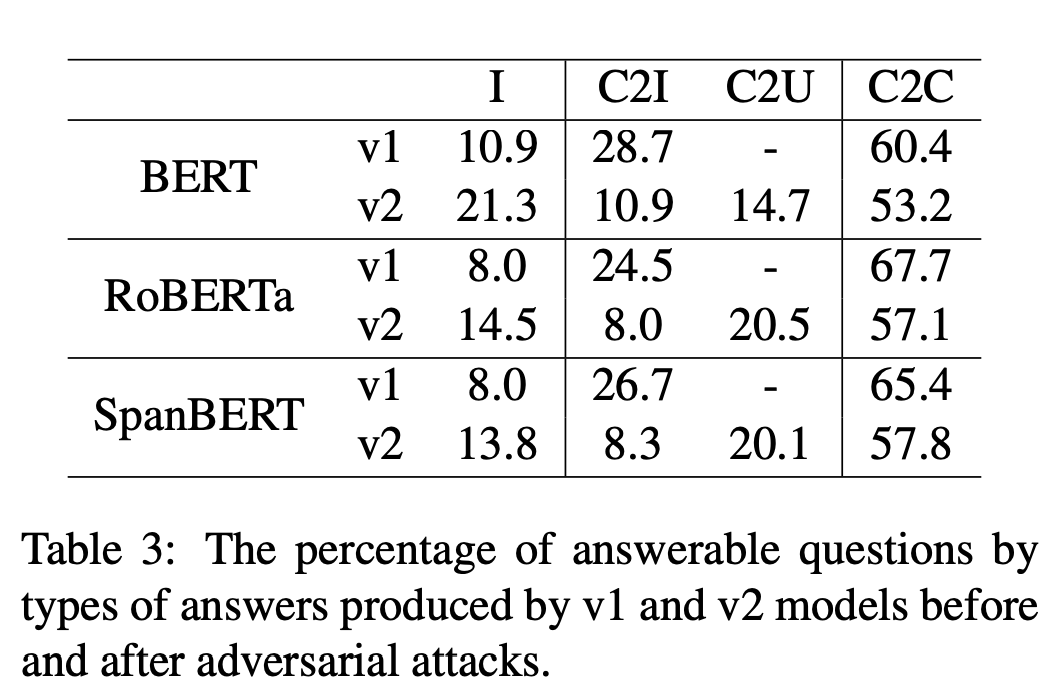
\includegraphics[width=0.5\textwidth]{figure1.png}
    \caption{Taken from the original paper \citep{impactsofunanswerable}}
    \label{fig:figure1}
\end{figure}

\begin{figure}[H]
    \centering
    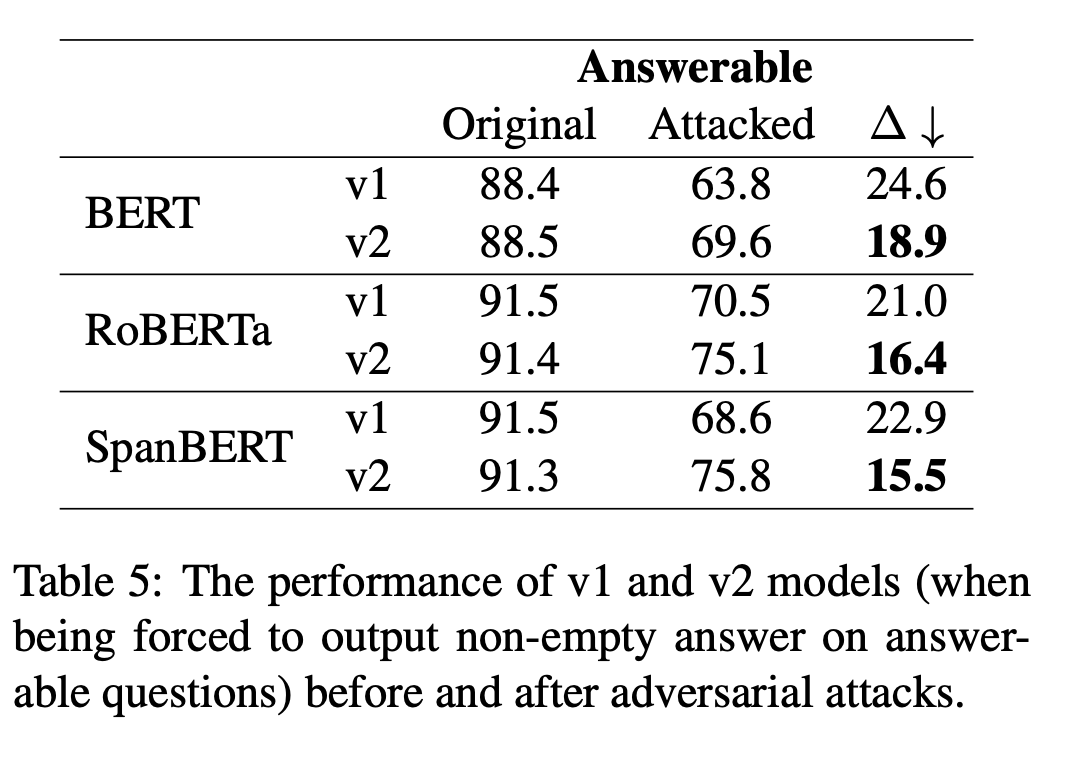
\includegraphics[width=0.5\textwidth]{figure2.png}
    \caption{Taken from the original paper \citep{impactsofunanswerable}}
    \label{fig:figure2}
\end{figure}

\begin{figure}[H]
    \centering
    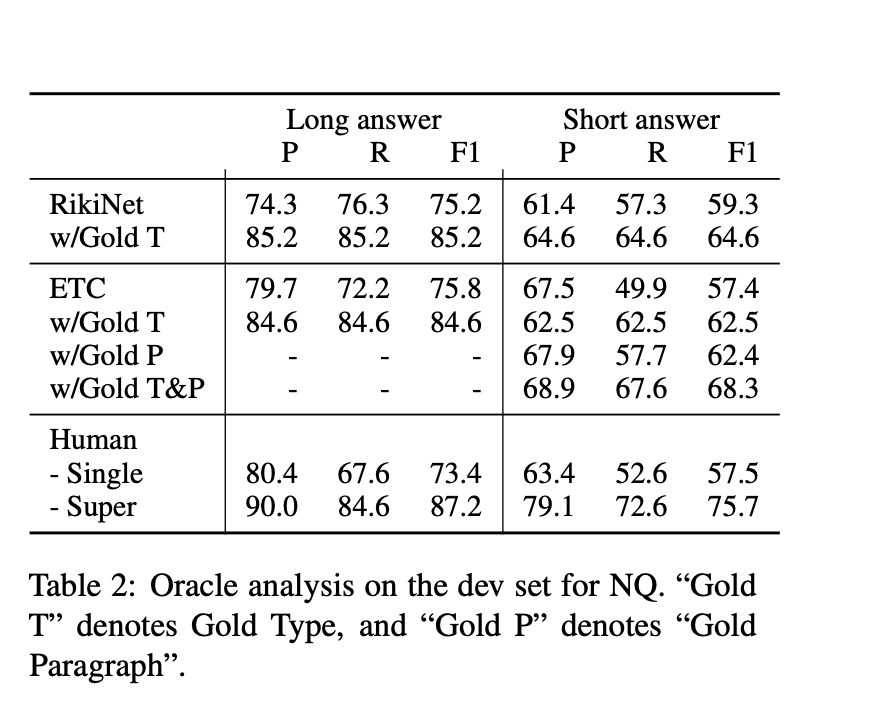
\includegraphics[width=0.5\textwidth]{figure3.png}
    \caption{Taken from the original paper \citep{informationseeking}}
    \label{fig:figure3}
\end{figure}

\bibliographystyle{acl_natbib}
\bibliography{main}
\end{document}
